% !TeX program = pdflatex
\documentclass[10pt,twocolumn]{article}

\usepackage[T1]{fontenc}
\usepackage[utf8]{inputenc}
\usepackage{lmodern}
\usepackage[margin=0.52in,top=0.49in,bottom=0.54in]{geometry}
\setlength{\columnsep}{0.19in}
\usepackage{amsmath,amssymb}
\usepackage{booktabs}
\usepackage{graphicx}
\usepackage{cite}
\usepackage{xurl}
\usepackage{xcolor}
\usepackage{microtype}
\usepackage{fancyhdr}
\usepackage{titlesec}
\usepackage[colorlinks=true,linkcolor=blue!60!black,citecolor=blue!60!black,urlcolor=blue!60!black,pdftitle={Static Structural Audit of the 17.37-Million-Line Lean 4 Riemann Hypothesis Archive: Trust Boundaries, Type-2 Clones, and Dependency Topology},pdfauthor={Chen Jiang}]{hyperref}

% =========================================================================
% Release Anchors
% =========================================================================
\newcommand{\zenodoDoi}{10.5281/zenodo.24465791}
\newcommand{\githubRepo}{https://github.com/Janson79jc/lean4-static-audit}
\newcommand{\archiveSha}{9631b4f020199e580ba86178cb56c6e9b09f690c2369a80dc4334aa93f49c7fc}
\newcommand{\archiveShaShort}{9631b4f02019}
\newcommand{\probeSha}{43501e2c8041ccdda6b59a4c324450c9f402c1913682be1f87d82d7562adfbce}
\newcommand{\probeShaShort}{43501e2c8041}

\newcommand{\ub}{\_\allowbreak}
\emergencystretch=3.5em
\tolerance=2000
\hbadness=2000
\linespread{0.96}

\renewcommand{\topfraction}{0.95}
\renewcommand{\bottomfraction}{0.85}
\renewcommand{\textfraction}{0.05}
\renewcommand{\dbltopfraction}{0.95}
\titlespacing*{\section}{0pt}{5pt plus 1pt minus 1pt}{2pt plus 1pt minus 1pt}
\titlespacing*{\subsection}{0pt}{4pt plus 1pt minus 1pt}{1.5pt plus 1pt minus 1pt}
\setlength{\textfloatsep}{5pt plus 1pt minus 1pt}
\setlength{\dbltextfloatsep}{5pt plus 1pt minus 1pt}
\setlength{\abovecaptionskip}{3pt}
\setlength{\belowcaptionskip}{1pt}

% Page 1 Cite-As Footer (Zenodo DOI) + clean running page numbers
\fancypagestyle{firstpage}{
  \fancyhf{}
  \renewcommand{\headrulewidth}{0pt}
  \renewcommand{\footrulewidth}{0.4pt}
  \fancyfoot[L]{\scriptsize\textbf{Cite as:} C.~Jiang (2026). \textit{Static Structural Audit of the 17.37-Million-Line Lean~4 Riemann Hypothesis Archive}. Zenodo. DOI: \href{https://doi.org/\zenodoDoi}{\texttt{\zenodoDoi}}. Code: Apache-2.0; Report/Data: CC~BY~4.0.}
  \fancyfoot[R]{\scriptsize\thepage}
}
\pagestyle{plain}

\title{\vspace{-1.8em}\Large\bfseries Static Structural Audit of the 17.37-Million-Line\\
Lean~4 Riemann Hypothesis Archive:\\
Trust Boundaries, Type-2 Clones, and Dependency Topology}

\author{\vspace{-0.4em}\normalsize Chen Jiang\\
\small Independent Researcher \quad $\cdot$ \quad \texttt{cjiang1@my.hpu.edu}\\
\small Artifacts: \href{\githubRepo}{\texttt{\githubRepo}} \quad $\cdot$ \quad Archive DOI: \href{https://doi.org/\zenodoDoi}{\texttt{\zenodoDoi}}}
\date{\vspace{-0.7em}\small November 23, 2026\vspace{-1.4em}}

\begin{document}
\maketitle
\thispagestyle{firstpage}

\begin{abstract}
Large-scale formal-mathematics repositories in Lean~4 increasingly exhibit the structural characteristics of ultra-large software systems, yet kernel type checking alone provides no visibility into forwarding-wrapper overhead, syntactic boilerplate, trust-boundary surface area, or module dependency concentration. We present a pure static, non-kernel empirical audit of a 175,187-file Lean~4 formalization archive (17,374,215 raw lines; 15,531,759 stripped code lines; 242,670 definitions and 818,755 theorems at column~0). Across the entire corpus, we find: (1)~\textbf{zero} detected occurrences across 17 checked lexical trust-boundary primitives (\texttt{sorry}, \texttt{admit}, \texttt{native\ub decide}, \texttt{@[extern]}, \texttt{@[csimp]}, \texttt{unsafe}, \texttt{axiom}), alongside \textbf{34} deduplicated \texttt{run\ub tac}/\texttt{liftMetaTactic}/\texttt{partial} sites (\textbf{64} raw hits) and \textbf{7} environment-mutation calls (\textbf{5} \texttt{modifyEnv}, \textbf{2} \texttt{addDecl}); (2)~exact separation of Type-2 proof clones (\textbf{20.51\%} overall) into forwarding shims (\textbf{96.27\%} duplication, with one 3-branch template \texttt{d52746a3d7614f9d} covering \textbf{43,525} of \textbf{50,682} shims, or \textbf{85.9\%}) versus substantive proofs $\ge 20$ tokens (\textbf{6.39\%} duplication, zero cross-bucket collisions); and (3)~\textbf{100.0\%} acyclic import reachability from \texttt{Main} (\textbf{753,261} edges, max depth \textbf{202}) coupled with pronounced structural skew (\texttt{transitive\ub blast\ub radius} Gini \textbf{0.8905}, Top 10\% holding \textbf{86.02\%}), where Top-30 blast-radius bottlenecks (\textbf{59.70\%--61.68\%} impact, direct fan-in \textbf{1--188}) are completely disjoint from Top-30 direct-fan-in hubs (\textbf{775--3,088} importers).

\medskip
\noindent\fbox{\parbox{0.96\linewidth}{\footnotesize\textbf{Hard Scope Disclaimer.} This audit performs purely static lexical, syntactic-pattern, and import-DAG analysis. It does \emph{not} re-run the Lean~4 or any external type-checking kernel, and neither certifies nor refutes the mathematical correctness of any theorem. Syntactic hits represent structural patterns rather than guaranteed defects; manual inspection confirms benign constructs such as legacy branch toggles (\texttt{SwOn.lean:3}) and base-case boundary predicates (\texttt{IsExpansion.lean:81}).}}
\end{abstract}

\section{Introduction and Corpus Snapshot}
Formal verification projects in Lean~4~\cite{Moura_2021} now scale to tens of millions of lines of code. For this November~2026 release, joint Lean~FRO and Mathlib~Initiative verification~\cite{LeanFRO_2026} independently certified statement fidelity and proof validity across multiple external checkers. Yet kernel pass/fail status leaves critical software-engineering questions unanswered: how much proof volume consists of substantive reasoning versus generated forwarding wrappers, where metaprogramming accesses the environment, how syntactic patterns correlate with module size, and how sensitive the import graph is under change propagation.

We audit the archived Lean~4 snapshot (toolchain \texttt{leanprover/lean4:v4.33.1}, \texttt{mathlib4} rev \texttt{0df444a3}) backed by immutable provenance:
\begin{itemize}\setlength{\itemsep}{1pt}\setlength{\parskip}{0pt}\setlength{\topsep}{2pt}
  \item \textbf{Source Archive}: \texttt{raw/lean.tar.gz} (239,275,554 bytes, SHA-256 \texttt{\archiveShaShort...}, full hash in \texttt{CITATION.cff} and JSON reports; flags \texttt{autoImplicit = false}, \texttt{maxHeartbeats = 4000000}).
  \item \textbf{Audit Probe Bundle}: \texttt{probe\ub bundle\ub sha256 = \probeShaShort...}, developed in a human--AI collaborative workflow and validated via 10 deterministic tests (\texttt{test\ub lean\ub probes.py}) plus conservation assertions (\texttt{invariants\ub checked.all\ub passed}).
  \item \textbf{Scale}: \textbf{175,187} \texttt{.lean} files, \textbf{17,374,215} raw lines, \textbf{15,531,759} stripped code lines (the 1,842,456-line gap consists solely of blank lines, with \textbf{0} comment-only lines), \textbf{242,670} definitions, and \textbf{818,755} theorems/lemmas (0 standalone \texttt{by trivial}; 20,023 \texttt{rfl}).
\end{itemize}

\section{Audit Pipeline and Methodology}
Our open-source pipeline executes four deterministic passes without modifying or executing target code; all counts are computed deterministically by script rather than model estimation:

\noindent\textbf{L1 (Comment/String-Safe Lexer).} Strips nested block comments (\texttt{/- ... -/}), line comments (\texttt{-\,-}), string literals, and escapes while preserving identifier characters including Unicode subscripts (e.g., \texttt{Bar\textsubscript{2}}, \texttt{x\textsubscript{1}}) and primes (\texttt{'}). Import extraction uses non-whitespace module matching so Unicode paths are never truncated.

\begin{figure*}[t]
\centering
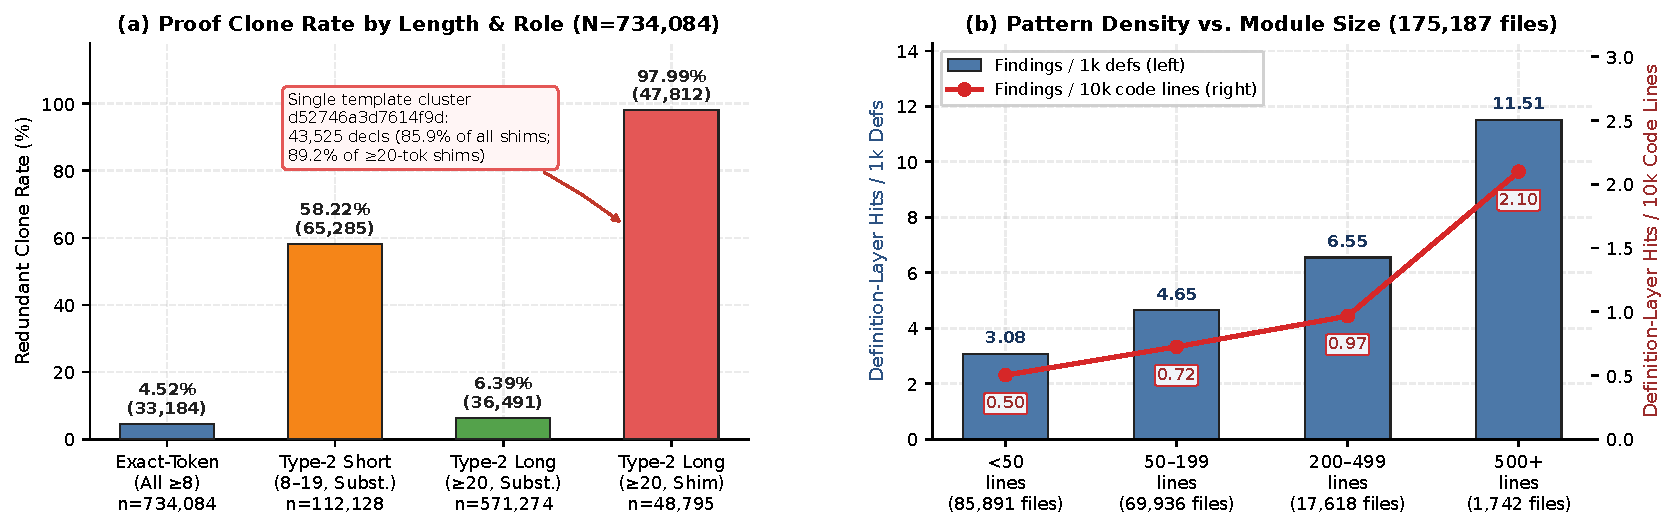
\includegraphics[width=0.70\textwidth]{../reports/figures/fig1_clones_and_density.pdf}
\caption{\textbf{Proof clone stratification and module-size pattern density.} (a)~Exact vs.\ Type-2 clone rates; bars~2--4 show the three primary Type-2 strata covering 99.7\% of eligible proofs (omitting the small 8--19 token shim stratum, $n=1{,}887$, 51.88\% duplication, detailed in Table~\ref{tab:clones}). (b)~Definition-layer syntactic pattern density per 1k definitions (bars) and per 10k code lines (curve) across non-empty file size buckets.}
\label{fig:clones}
\end{figure*}

\noindent\textbf{L2 (Column-0 Parser, Probes, and Clone Normalization).} Parses top-level column-0 declarations (\texttt{def}, \texttt{abbrev}, \texttt{structure}, \texttt{class}, \texttt{instance}, \texttt{inductive}, \texttt{theorem}, \texttt{lemma}), masking balanced inline \texttt{(by ...)} and indentation-scoped tactic subblocks before scanning definition terms. For bodies with $\ge 8$ tokens, we compute SHA-256 hashes under (i)~\emph{Exact-Token} matching and (ii)~\emph{Type-2 Parameterized Identifier Normalization}~\cite{Roy_2009}, which preserves Lean keywords, core tactics, operators, and numeric literals while renaming all other identifiers consistently (\texttt{V0}, \texttt{V1}, \dots). Proofs are partitioned into \emph{forwarding shims}---bodies matching \texttt{(by )?(first | | exact )} without non-forwarding tactics (\texttt{have}, \texttt{let}, \texttt{rw}, \texttt{simp}, \texttt{ring}, \texttt{linarith}, \texttt{ext}, etc., via dot-safe lookarounds)---and \emph{substantive proofs}.

\noindent\textbf{L2.5 (Extended Trust \& Dual Scan).} Scans masked source for kernel/compiler primitives (including combined attributes \texttt{@[inline, extern]}, \texttt{@[simp, csimp]}, \texttt{attribute [csimp]}, and \texttt{addDeclCore}/\texttt{addDeclWithoutChecking}), metaprogramming entry points (\texttt{run\ub tac}, \texttt{liftMetaTactic}, \texttt{run\ub cmd}, \texttt{elab}, \texttt{macro}, \texttt{initialize}, \texttt{import [all] Lean}), logical duals (\texttt{False} predicates, dummy witnesses), and target shadowing (\texttt{configs/rh\ub archive.json}).

\noindent\textbf{L3-A \& SE Topology.} Deduplicates import edges, verifies DAG acyclicity and reachability from \texttt{Main}, computes exact transitive blast radius across all 175,187 modules via chunked topological bitsets, and evaluates Gini concentration across size, declaration, and coupling distributions.

\section{Empirical Findings}

\subsection{Trust-Boundary and Metaprogramming Inventory}
Across all 175,187 files, zero occurrences of the 17 checked lexical trust-boundary primitives were detected in comment/string-masked source (Table~\ref{tab:trust}): \texttt{sorry}, \texttt{admit}, \texttt{sorryAx}, \texttt{mkSorry}, \texttt{native\ub decide}, \texttt{ofReduceBool}, \texttt{ofReduceNat}, \texttt{implemented\ub by}, \texttt{@[extern]}, \texttt{@[csimp]}, \texttt{debug.skipKernelTC}, \texttt{trustCompiler}, \texttt{unsafe}, \texttt{axiom}, \texttt{opaque}, \texttt{addAndCompile}, and \texttt{setEnv} all measure \textbf{0}.

Metaprogramming and environment-access activity is tightly localized, with all non-macro high-signal sites exhaustively inspected: \textbf{34} deduplicated \texttt{run\ub tac}/\texttt{liftMetaTactic}/\texttt{partial} locations correspond to \textbf{64} raw hits (\texttt{run\ub tac = 32}, \texttt{liftMetaTactic = 30}, \texttt{partial\ub def = 2}), plus \textbf{7} source-level environment mutation calls: \textbf{5} \texttt{modifyEnv} calls in \texttt{BuildAid/D1..D5.lean} (each paired with \texttt{run\ub cmd} appending to \texttt{LibrarySuggestions.nameDenyListExt}) and \textbf{2} \texttt{addDecl} calls in \texttt{CutCptCopy.lean}. All \textbf{12} direct \texttt{import [all] Lean} lines appear in 7 helper files (\texttt{BuildAid/D1..D5.lean}: 10; \texttt{Imports.lean}: 1; \texttt{OwnStruct.lean}: 1), whereas \texttt{CutCptCopy.lean} accesses \texttt{Lean} via transitive imports and accounts for 1 of the \textbf{4} \texttt{elab} commands. The \textbf{87} \texttt{macro}/\texttt{macro\ub rules} declarations across 64 files were spot-checked; sampled instances are local \texttt{scoped macro} proof shorthands.

\begin{table}[t]
\centering
\caption{Trust-Boundary \& Metaprogramming Inventory (175,187 Files)}
\label{tab:trust}
\footnotesize
\setlength{\tabcolsep}{3.0pt}
\resizebox{\columnwidth}{!}{%
\begin{tabular}{@{}lr@{\hspace{8pt}}lr@{}}
\toprule
\textbf{Category / Primitive} & \textbf{Count} & \textbf{Category / Primitive} & \textbf{Count} \\
\midrule
\texttt{sorry}/\texttt{admit}/\texttt{sorryAx}/\texttt{mkSorry} & 0 & \texttt{run\ub tac}/\texttt{liftMeta}/\texttt{partial} & 32/30/2 \\
\texttt{native\ub decide}/\texttt{ofReduce*} & 0 & Deduplicated sites of 3 above & 34 \\
\texttt{implemented\ub by}/\texttt{extern}/\texttt{csimp} & 0 & \texttt{modifyEnv} (\texttt{BuildAid/D1..D5}) & 5 \\
\texttt{skipKernelTC}/\texttt{trustCompiler} & 0 & \texttt{addDecl} (\texttt{CutCptCopy.lean}) & 2 \\
\texttt{unsafe}/\texttt{axiom}/\texttt{opaque} & 0 & \texttt{run\ub cmd}/\texttt{elab}/\texttt{macro} & 5/4/87 \\
\texttt{addAndCompile}/\texttt{setEnv}/\texttt{init} & 0 & \texttt{import [all] Lean} (7 files) & 12 \\
\bottomrule
\end{tabular}%
}
\end{table}

\subsection{Type-2 Clones and Single-Template Dominance}
\begin{figure*}[t]
\centering
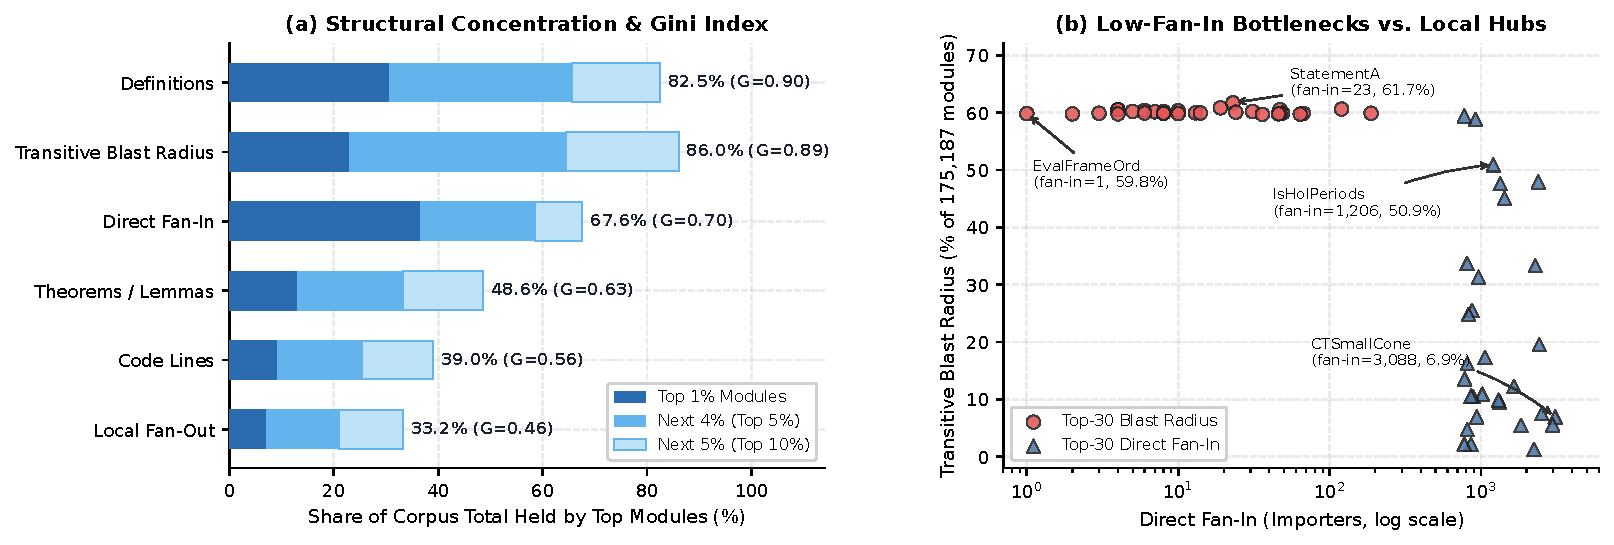
\includegraphics[width=0.70\textwidth]{../reports/figures/fig2_topology_concentration.pdf}
\caption{\textbf{Structural concentration and bottleneck separation.} (a)~Share of corpus totals held by Top~1\% / 5\% / 10\% modules with Gini coefficients. (b)~Log direct fan-in vs.\ transitive blast radius (\%) for Top-30 blast-radius hubs (circles, fan-in 1--188, 59.70\%--61.68\%) and Top-30 direct-fan-in hubs (triangles, fan-in 775--3,088, 1.28\%--59.42\%, topped by \texttt{LocTied} at 59.42\% and \texttt{RhoDetPrimeEqMuTildeMulChiPow} at 58.80\%); the two Top-30 sets are completely disjoint.}
\label{fig:topo}
\end{figure*}
Applying Type-2 normalization raises aggregate proof duplication from \textbf{4.52\%} (Exact-Token) to \textbf{20.51\%} (\textbf{150,567} redundant declarations across \textbf{35,921} clusters; Table~\ref{tab:clones}). Crucially, stratifying by role and token length eliminates cross-bucket collisions (\textbf{0} overlap) and reveals two contrasting regimes (Fig.~\ref{fig:clones}(a)):

\begin{itemize}\setlength{\itemsep}{1pt}\setlength{\parskip}{0pt}\setlength{\topsep}{2pt}
  \item \textbf{Forwarding Shims Collapse to Boilerplate.} Among \textbf{50,682} forwarding shims ($\ge 8$ tokens), \textbf{96.27\%} (\textbf{48,791}) are Type-2 duplicates across only \textbf{277} clusters; at $\ge 20$ tokens, duplication reaches \textbf{97.99\%} (\textbf{47,812 / 48,795} across \textbf{87} clusters). A \emph{single} template cluster (\texttt{d52746a3d7614f9d}: \texttt{first | exact @T | exact T | (intros; apply T <;> assumption)}, e.g., \texttt{BesselCayleySideBoundStatement.lean:16--17}) accounts for \textbf{43,525} declarations---\textbf{85.9\%} of all shims and \textbf{89.2\%} of $\ge 20$-token shims.
  \item \textbf{Long Substantive Proofs Are Diverse.} Substantive proofs $\ge 20$ tokens (\textbf{571,274} declarations) drop to \textbf{6.39\%} Type-2 duplication (\textbf{36,491} duplicates across \textbf{24,109} clusters, max cluster size \textbf{144}, zero clusters $>500$, compared to \textbf{8.34\%} for $\ge 20$-token definitions). Short substantive proofs (8--19 tokens) supply most non-shim repetition (\textbf{58.22\%}, \textbf{65,285} duplicates). Across all Type-2 substantive clusters (\textbf{35,644}), \textbf{26.6\%} (\textbf{9,487}) span multiple top-level directories, \textbf{59.5\%} (\textbf{21,191}) span files within a top-level directory, and \textbf{13.9\%} (\textbf{4,966}) are single-file local.
\end{itemize}

\begin{table}[t]
\centering
\caption{Clone Decomposition ($\ge 8$ Tokens; Zero Cross-Bucket Overlap)}
\label{tab:clones}
\footnotesize
\setlength{\tabcolsep}{3.0pt}
\resizebox{\columnwidth}{!}{%
\begin{tabular}{@{}llrrr@{}}
\toprule
\textbf{Mode / Tokens} & \textbf{Layer} & \textbf{Eligible} & \textbf{Clusters} & \textbf{Dup (\%)} \\
\midrule
Exact ($\ge 8$) & Definition & 204,234 & 7,767 & 10,646 (5.21\%) \\
Exact ($\ge 8$) & Proof (All) & 734,084 & 22,941 & 33,184 (4.52\%) \\
\midrule
Type-2 ($\ge 8$) & Definition & 204,234 & 15,544 & 33,294 (16.30\%) \\
Type-2 ($\ge 8$) & Proof (All) & 734,084 & 35,921 & 150,567 (20.51\%) \\
Type-2 ($\ge 20$) & Definition & 149,870 & 8,766 & 12,502 (8.34\%) \\
Type-2 (8--19) & Proof Shim & 1,887 & 190 & 979 (51.88\%) \\
Type-2 (8--19) & Proof Subst. & 112,128 & 11,535 & 65,285 (58.22\%) \\
Type-2 ($\ge 20$) & Proof Shim & 48,795 & 87 & 47,812 (97.99\%) \\
Type-2 ($\ge 20$) & Proof Subst. & 571,274 & 24,109 & 36,491 (6.39\%) \\
\bottomrule
\end{tabular}%
}
\end{table}

\subsection{Definition-Layer Patterns, Enrichment, and Scaling}
We detect \textbf{1,403} definition-layer pattern hits, all reachable within the \texttt{Main} entry cone: \texttt{DEF\ub UNUSED\ub EXPLICIT\ub UNDERSCORE\ub PARAM} (\textbf{881}), \texttt{DEF\ub UNUSED\ub EXPLICIT\ub NAMED\ub PARAM} (\textbf{210}), \texttt{DEF\ub SINGLEARG\ub FUN\ub TRUE} (\textbf{162}), \texttt{DEF\ub EXPLICIT\ub WILDCARD\ub PARAM} (\textbf{77}), \texttt{DEF\ub MULTIARG\ub FUN\ub TRUE} (\textbf{54}), \texttt{DEF\ub FUN\ub TRUE} (\textbf{9}), \texttt{DEF\ub CONST\ub TRUE} (\textbf{8}), and \texttt{DEF\ub TRIVIAL\ub STUB} (\textbf{2}), plus \textbf{1,218} informational theorem-signature \texttt{fun \_+ => True} hits. Hits concentrate disproportionately in \texttt{Formalism/} (18,254 files, 18.0\% of code lines), which holds \textbf{63.6\%} (892/1,403) of findings at \textbf{3.20} / 10k lines (\textbf{11.44} / 1k defs)---\textbf{7.8$\times$} by lines and \textbf{3.3$\times$} by defs over \texttt{Development/} (457 hits; 0.41 / 10k lines, 3.50 / 1k defs). Across file size buckets (Fig.~\ref{fig:clones}(b)), hit density climbs \textbf{3.74$\times$} per def (3.08$\to$11.51) and \textbf{4.20$\times$} per line (0.50$\to$2.10). L2.5 checks add \textbf{17} parameterized dummy constants, \textbf{1} \texttt{DEF\ub CONST\ub FALSE} (\texttt{SwOn.lean:3}), \textbf{1} \texttt{DEF\ub FUN\ub FALSE} (\texttt{IsExpansion.lean:81}), and \textbf{8} symbol shadowings (0 for \texttt{RiemannHypothesis}, \texttt{GRH}, or \texttt{riemannZeta}; the 8 hits are the 4 canonical statement definitions in \texttt{Statements.lean} plus 2 local \texttt{ZeroFree} and 2 local \texttt{LFunction} definitions).

\subsection{Dependency Topology, Skew, and Hub Bottlenecks}
Every file (\textbf{175,187 / 175,187}, \textbf{100.0\%}) is reachable from \texttt{Main} via \textbf{753,261} deduplicated import edges forming a strict acyclic DAG (\texttt{max\ub depth = 202}, \texttt{p90 = 98}; \textbf{174} zero-declaration files). While \texttt{Development} (\textbf{141,928} files) drives inward edges to \texttt{Development} (\textbf{577,034}), \texttt{Formalism} (\textbf{41,857}), and \texttt{ReciprocityTheory} (\textbf{38,051}), reverse directory-level coupling edges exist: \texttt{Formalism} $\to$ \texttt{Development} (\textbf{236}), \texttt{Formalism} $\to$ \texttt{ReciprocityTheory} (\textbf{348}), \texttt{GroundTheory} $\to$ \texttt{Development} (\textbf{57}), and \texttt{ReciprocityTheory} $\to$ \texttt{Development} (\textbf{17}).

Structural skew is pronounced (Table~\ref{tab:topo}, Fig.~\ref{fig:topo}(a)): definitions reach Gini \textbf{0.8989} (Top 10\% hold \textbf{82.45\%}) and \texttt{transitive\ub blast\ub radius} reaches Gini \textbf{0.8905} (Top 10\% hold \textbf{86.02\%}). Paralleling the centrality divergence between infrastructural and mathematical modules observed in Mathlib~\cite{Li202624797}, Fig.~\ref{fig:topo}(b) shows a complete separation between local popularity and global impact: Top-30 blast-radius hubs (\textbf{59.70\%--61.68\%}, led by \texttt{Formalism.RealPlaceAnalysis.StatementA} at \textbf{108,056} modules with fan-in \textbf{23}, and \texttt{EvalFrameOrd} at \textbf{59.81\%} with fan-in \textbf{1}) all have fan-in \textbf{1--188} and are \emph{100\% disjoint} from Top-30 direct-fan-in hubs (\textbf{775--3,088} importers, \textbf{1.28\%--59.42\%} blast radius, from \texttt{CTSmallCone} at \textbf{6.91\%} up to \texttt{IsHolPeriods} at \textbf{50.90\%} and \texttt{LocTied} at \textbf{59.42\%}).

\begin{table}[t]
\centering
\caption{Corpus Concentration and Quantiles (175,187 Modules)}
\label{tab:topo}
\footnotesize
\setlength{\tabcolsep}{3.0pt}
\begin{tabular}{@{}lrrrrrr@{}}
\toprule
\textbf{Metric} & \textbf{Gini} & \textbf{Top 1\%} & \textbf{Top 10\%} & \textbf{P50} & \textbf{P90} & \textbf{Max} \\
\midrule
Code Lines & 0.5631 & 9.14\% & 39.03\% & 51 & 210 & 14,814 \\
Definitions & 0.8989 & 30.65\% & 82.45\% & 0 & 3 & 226 \\
Theorems & 0.6273 & 13.10\% & 48.59\% & 1 & 12 & 1,518 \\
Direct Fan-In & 0.6966 & 36.63\% & 67.62\% & 1 & 5 & 3,088 \\
Local Fan-Out & 0.4626 & 7.03\% & 33.20\% & 3 & 9 & 370 \\
Blast Radius & 0.8905 & 22.93\% & 86.02\% & 87 & 6,888 & 108,056 \\
\bottomrule
\end{tabular}
\end{table}

\section{Threats to Validity and Conclusion}
\noindent\textbf{Construct, Scope, and Verification Boundaries.} Our scanning operates strictly on comment/string-masked \texttt{.lean} source text; it does \emph{not} inspect post-macro-expansion elaborated terms, \texttt{lakefile} build scripts, or external FFI binaries. Our column-0 parser excludes definitions inside \texttt{mutual} blocks, indented \texttt{namespace}/\texttt{section} scopes, and equational pattern-matching \texttt{def}s without \texttt{:=} from declaration counts. Forwarding-shim classification is syntactic; the 97.99\% collapse of $\ge 20$-token shims (89.2\% in one pattern) is consistent with high precision. Because the Python probes were developed in a human--AI workflow without line-by-line manual Python audit, verification rests on 10 deterministic tests, pre-output conservation invariants, and hashed script archival (\texttt{\probeShaShort...}); manual Lean inspection focused on flagged high-signal targets (\texttt{SwOn.lean:3}, \texttt{IsExpansion.lean:81}, and environment-mutation sites).

\noindent\textbf{Conclusion and Availability.} At 17.37M raw lines, this Lean~4 snapshot shows zero detected lexical trust escapes, sharp separation between boilerplate forwarding wrappers (\textbf{43,525} copies of one pattern) and diverse long proofs (\textbf{6.39\%} Type-2 duplication), and high topological concentration (\textbf{0.8905} blast-radius Gini). All audit and plotting scripts (\texttt{scripts/}, \texttt{configs/}; Apache-2.0), along with aggregate JSON/Markdown reports, figures, and this paper (CC~BY~4.0), are archived at \href{\githubRepo}{\texttt{\githubRepo}} and Zenodo (\href{https://doi.org/\zenodoDoi}{\texttt{\zenodoDoi}}). An extended study covering elaboration-level symbol-cone replay and cross-repository longitudinal comparisons is currently in preparation.

\bibliographystyle{IEEEtran}
{\footnotesize\sloppy
\bibliography{refs}
}
\end{document}
